\chapter{Paradoxes, Thought Experiments, and the Illusions}
A \newterm{paradox} is a statement that contradicts itself or defies intuition. Paradoxes often arise in mathematics, physics, and philosophy, challenging our realities and understanding of reality and logic. \index{paradox}

We are going to talk about them here to introduce the idea of proofs by contradiction, which is a powerful tool in mathematics. A proof by contradiction assumes that the statement we want to prove is false and then shows that this assumption leads to a logical contradiction. We are also going to talk about a multitude of paradoxes in fields such as mathematics, physics, and architecture.

Some of these will also be \newterm{thought experiments}. Thought experiments involve considering an imaginary scenario that tests a theory or argument, and many times, one that would be rare or impossible to test. Scientists use this to refute past (incorrect) knowledge, establish new theories, or even provide scenarios about human nature\footnote{\url{https://en.wikipedia.org/wiki/Trolley_problem}}. Doing this allows engineers to isolate variables, look at edge cases, improve intution of what \textit{should} happen, and consider how breakthroughs could occur. In fact, Isaac Newton used a thought experiment comparing a falling apple and the Moon to help develop his theory of universal gravitation (recall the Newton's cannon idea). In many of our physics scenarios, we imagine a \textit{frictionless surface}. This will never truly exist, all materials involve some sort of friction, so we consider this a thought experiment

If you recall, we talked in the proofs chapter about the different types of proofs, specifically proofs by contradiction. We will now talk about some examples of proofs by contradiction, and how they relate to paradoxes. We will use proofs by contradiction to prove many of our paradoxes.

The Barber's Paradox is a self-referential paradox that arises in set theory and logic.

The paradox is often stated as follows
\begin{theorem}
    In a town, there is a barber who shaves all and only those men who do not shave themselves. The question is: Does the barber shave himself?
\end{theorem}
Well there are two cases to consider:
\begin{itemize}
    \item If the barber shaves himself, then according to the definition, he is now someone who \textit{shaves himself}. The rule says the barber only shaves people who do not shave themselves. This is a contradiction because the barber cannot both shave himself and not shave himself at the same time.
    \item If the barber does not shave himself, then according to the definition, he is someone who does not shave himself. The rule says the barber shaves all those who do not shave themselves. This means the barber must shave himself, which again leads to a contradiction because he cannot both shave himself and not shave himself at the same time.
\end{itemize}
The reason this is a paradox is that no matter which path you take, you end up at a contradiction. The barber cannot exist under those rules. A paradox will often arise from statements that are self-referential or involve circular definitions, which is the case here. It is important to note that some paradoxes that we will talk about will have resolutions, but the Barber's Paradox is an example of a paradox that does not have a resolution.

In proofs by contraction we often intentionally create a contradiction to prove a theorem. In the Barber's Paradox, we assumed the two possible cases for the barber (shaving himself or not shaving himself) and showed that both lead to a contradiction.

\section{Mathematical Paradoxes}
\subsection{Russell's Paradox}\index{Russell's Paradox}\index{set theory}
Russell's Paradox is a paradox within set theory. It arises from the statement that
\begin{theorem}
    Consider the set of all sets that do not contain themselves. Does this set contain itself?
\end{theorem}
Let's consider some simple sets. The set of all apples \emph{is not} an apple, it is a list of apples. Similarly, the set of all of ideas \emph{is} an idea, it is a concept.
For Russell's statement, let's create a master set $R$ that contains only the sets that do not contain themselves. There are two cases:
\begin{itemize}
    \item If $R$ is not a member of itself, then its definition entails that it is a member of itself. $\rightarrow \leftarrow$
    \item If $R$ is a member of itself, then it is not a member of itself, since it is the set of all sets that are not members of themselves. $\rightarrow \leftarrow$
\end{itemize}
Using symbols from our sets chapter,
\[\text{Let } R = \{x | x \not \in x\}\text{. Then }  R\in R\iff R\not \in R. \text{This is a } \rightarrow \leftarrow\]

\subsection{Simpson's Paradox}
Simpson's Paradox is a phenomenon in statistics where a trend or correlation that appears in several different groups of data can disappear or reverse when the groups are combined. Let's look at an example.\index{Simpson's paradox}

Imagine we are comparing two hospitals, Hospital A and Hospital B, for their success rates in completing a operational surgery. We have the following data:

\begin{table}[!ht]
    \centering
    \begin{tabular}{|l|l|l|l|}
        \hline
        \textbf{Hospital} & \textbf{Total Patients} & \textbf{Survived} & \textbf{Survival Rate} \\ \hline
        Hospital A        & 1000                    & 800               & 80\%                   \\ \hline
        Hospital B        & 1000                    & 890               & 89\%                   \\ \hline
    \end{tabular}
\end{table}

From this, we see that the same number of patients were treated at both hospitals, but Hospital B has a higher survival rate. This would lead us to think that Hospital B is the better hospital, due to money, education of doctors, or whatever factor. However, let's look at the data when seperated by those with \textit{high-risk} surgeries versus those with \textit{low-risk} surgeries.

Patients that had low-risk surgeries, or were in good health, are given by following data
\begin{table}[H]
    \centering
    \begin{tabular}{|l|l|l|l|}
        \hline
        \textbf{Hospital} & \textbf{Patients} & \textbf{Survived} & \textbf{Survival Rate} \\ \hline
        Hospital A        & 100               & 98                & 98\%                   \\ \hline
        Hospital B        & 900               & 850               & 94.4\%                 \\ \hline
    \end{tabular}
\end{table}
And those with poor health and high-risk surgeries:
\begin{table}[H]
    \centering
    \begin{tabular}{|l|l|l|l|}
        \hline
        \textbf{Hospital} & \textbf{Patients} & \textbf{Survived} & \textbf{Survival Rate} \\ \hline
        Hospital A        & 900               & 702               & 78\%                   \\ \hline
        Hospital B        & 100               & 40                & 40\%                   \\ \hline
    \end{tabular}
\end{table}

Looking at the data based on the health categorization, Hospital A is actually better in both categories. This ``paradox'' occurs due the unaccounted, \textbf{independent variable}: the incoming health of the patient. Hospital A took on the harder cases (90\% of their patients are high-risk). Hospital B, although it initially was thought to be the better hospital, mainly took on those with good health (90\% were low-risk).

For fun, let's plot this using pandas and matplotlib libraries in Python. The code is as follows:
\begin{minted}{python}
import pandas as pd
import matplotlib.pyplot as plt
import seaborn as sns

# aggregate the data
data = {
    'Condition': ['Good', 'Good', 'Poor', 'Poor', 'Total', 'Total'],
    'Hospital': ['A', 'B', 'A', 'B', 'A', 'B'],
    'Survival': [0.98, 0.94, 0.78, 0.40, 0.80, 0.89]
}
df = pd.DataFrame(data)

# split into subgroups and totals for showing different correlations
subgroups = df[df['Condition'] != 'Total']
totals = df[df['Condition'] == 'Total']


fig, (ax1, ax2) = plt.subplots(1, 2, figsize=(10, 5), sharey=True)
# regression lines and plots 
ax1.plot([-0.2, 0.8], [0.98, 0.78], 'b--', marker='o', label='Trend A') 
ax1.plot([0.2, 1.2], [0.94, 0.40], 'y--', marker='o', label='Trend B') 
ax1.legend()
ax2.plot([-0.2, 0.2], [0.80, 0.89], 'k-', marker='o', label='Overall Trend')
ax2.legend()
sns.barplot(data=subgroups, x='Condition', y='Survival', hue='Hospital', ax=ax1)
ax1.set_title('Subgroups (A Wins)')

sns.barplot(data=totals, x='Condition', y='Survival', hue='Hospital', ax=ax2)
ax2.set_title('Total (B Wins)')

plt.tight_layout()
plt.show()
\end{minted}
This creats two bar plots with opposing regression lines:
\begin{figure}[H]
    \centering
    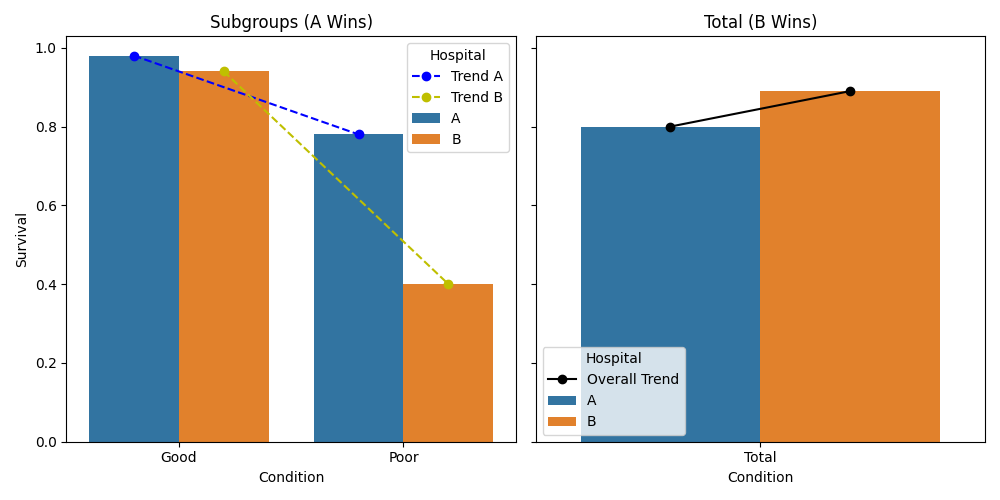
\includegraphics[width=0.8\textwidth]{hospitals.png}
    \caption{Simpson's Paradox: Subgroups vs. Total}
    \label{fig:simpsons}
\end{figure}
\subsection{Monty Hall Problem}
Watch the following video the introduce the \href{https://www.youtube.com/watch?v=cXqDIFUB7YU}{Monty Hall Problem}.\index{Monty Hall Problem}

The problem is as follows:
\begin{theorem}
    You are on a game show and are given the choice of three doors. Behind one door is a car; behind the others, goats. You pick a door, say No. 1, and the host, who knows what's behind the doors, opens another door, say No. 3, which has a goat. He then says to you, ``Do you want to switch to door No. 2?'' Is it to your advantage to switch your choice?
\end{theorem}

ADD: an adobe illustration of the doors and the host opening one of them, and the probabilities of each door having the car after the host opens one.

Your choice of Door No. 1 has a 1/3 chance of being the car and a 2/3 chance of being a goat. When the host opens Door No. 3, which has a goat, the probability of each door changes! Even though there are two doors left, the probability is \textit{50/50}. The probability of the car being behind Door No. 1 remains 1/3, while the probability of the car being behind Door No. 2 \emph{increases to 2/3}. Therefore, it is to your advantage to switch to Door No. 2, as it has a higher probability of containing the car.


\subsection{Birthday Problem}
The birthday problem is a famous problem in probability and combinatorics. It goes as follows:
\begin{theorem}
    In a group of $n$ people, what is the probability that at least two people share the same birthday?
\end{theorem}
The answer is often surprising to people because it is much higher than most people expect. Only $23$ people are needed to guarantee a \textit{majority}, where greater than $50\%$ chance that at least two people share a birthday. Let's prove this.

Let $P(A)$ the probability that a group of $k$ people do \emph{not} share a birthday. Further, let $P(B) = \neg P(A)= 1 - P(A)$ be the probability that at least two people share a birthday. We want to find the smallest $k$ such that $P(B) > 0.5$, as this constitutes a majority.

If there are only two people in a room(meaning $k=2$), the probability that there does not exist a shared birthday is $P(A) = \tfrac{364}{365}$, meaning the probability that there is a shared birthday is $P(B) = 1 - P(A) = \tfrac{1}{365}$. If there are three people in a room, the probability that there does not exist a shared birthday is $P(A) = \tfrac{364}{365} \cdot \tfrac{363}{365}$, meaning the probability that there is a shared birthday is $P(B) = 1 - P(A) = 1 - \tfrac{364}{365} \cdot \tfrac{363}{365}$.

This pattern continues, and we can generalize the probability that there does not exist a shared birthday for $k$ people as follows:
\[P(A) = \frac{365}{365} \cdot \frac{364}{365} \cdot \frac{363}{365} \cdots \frac{365-k+1}{365} = \prod_{i=0}^{k-1} \frac{365 - i}{365}.\]
Therefore, the probability that there is at least one shared birthday is:
\[P(B) = 1 - P(A) = 1 - \prod_{i=0}^{k-1} \frac{365 - i}{365}.\]

We now seek the smallest $k$ such that
\[
    1-\prod_{i=0}^{k-1}\frac{365-i}{365} > 0.5.
\]
Equivalently,
\[
    \prod_{i=0}^{k-1}\frac{365-i}{365} < 0.5.
\]

Computing this product gives
\[
    P(A)\approx 0.5073 \quad \text{when } k=22,
\]
so
\[
    P(B)\approx 1-0.5073=0.4927<0.5.
\]
But for $k=23$,
\[
    P(A)\approx 0.4927,
\]
so
\[
    P(B)\approx 1-0.4927=0.5073>0.5.
\]

Thus, the smallest number of people needed so that the probability of at least two sharing a birthday exceeds $50\%$ is $23$ people. Much smaller than most people expect!

\subsection{Zeno's Paradoxes}
Zeno was a Greek philosopher who is famous for his paradoxes, who created challenging thought experiments and paradoxes that question our understand of motion, space, physics, and time. Zeno's paradoxes are often used to illustrate the concept of \textit{infinity} and the nature of space and time.

\subsubsection{The Dichotomy Paradox}
His most famous paradoxes include is called the \textit{Dichotomy Paradox}, which he stated as
\begin{quote}
    That which is in locomotion must arrive at the half-way stage before it arrives at the goal.
\end{quote}
This paradox suggests that before an object can reach its destination, it must first reach the halfway point, and before it can reach the halfway point, it must reach the quarter point, and so on, leading to an infinite number of steps that must be completed before reaching the destination. This seems to imply that motion is impossible, as it would require completing an infinite number of tasks in a finite amount of time.

So then, how is motion possible?

The resolution to Zeno's paradoxes lies in the concept of limits and infinite series. In modern mathematics, we understand that an infinite number of steps can be completed in a finite amount of time if the steps get smaller and smaller. If we consider the remaining distance to be covered as $1 \, \mathrm{unit}$, the first step is $\frac{1}{2}$, the second step is $\frac{1}{4}$, the third step is $\frac{1}{8}$, and so on. The total distance covered after $n$ steps can be expressed as a geometric series:
\[
    S = \sum_{n=1}^{\infty} \frac{1}{2^n} = 1
\]
For proof's sake, let
$$S = \frac{1}{2} + \frac{1}{4} + \frac{1}{8} + \cdots$$
Then, multiplying both sides by $\frac{1}{2}$ gives
$$\frac{1}{2}S = \frac{1}{4} + \frac{1}{8} + \frac{1}{16} + \cdots$$
$$S - \frac{1}{2}S = \frac{1}{2}$$
$$\frac{1}{2}S = \frac{1}{2}    \quad \implies \quad    S = 1$$


\section{Physics and Time Travel Paradoxes}
A lot of what we have touched are counter-intuitive mathematical equations. Now we can look at some physics paradoxes and thought experiments that may mess with your brain a bit. A lot of these actually involve a concept called superposition.

\section{Schrödinger's Cat}
Erwin Schrödinger was a physicist with thoughts on quantum superposition, subatomic events, and early quantum theory. This thought experiment arose in a discussion with Albert Einstein, Niels Bohr, and Werner Heisenberg, all physicists from Europe working towards quantum development.

The thought experiment is as follows:
\begin{quote}
    Schrödinger imagined placing a cat in a sealed box with a device triggered by a quantum event (such as the decay of an atom, which depends on an electron-level process, or radioactive gunpowder, which Einstein preferred). The event has a 50\% chance of happening and a 50\% chance of staying dormant. If the event occurs, the cat dies; if not, it lives. However, you do not know whether the cat is alive or not until the box is opened. Schrödinger states that, the moment before the box is opened, the cat is equal parts dead and alive.
\end{quote}
Why is this? Well, the cat, in Schrödinger's world, is theoretically governed by quantum physics and quantum position. \textbf{Quantum Superposition} states that an object, usually an electron, exists in a \textbf{superposition of states}, such that it occupies multiple positions or energy states until it is measured. Before measurement, the electron is not in one definite state; instead, it is described by a wavefunction that encodes multiple possibilities simultaneously. If electrons are fired at a barrier with two narrow slits and then detected on a screen behind it, they produce an interference pattern, one with alternating covered and uncovered regions. This is characteristic of wave behavior, showing that electrons are travelling in waves. Further, when we talk about nonpolar covalent bonds, the electrons are present in both atoms simutaneously. \index{superposition}\index{Schrödinger's cat}

We say that the cat is in a superposition of both equally possible dead or alive states. There is a great video on Schrödinger's Cat and its relation to quantum physics by TedEd in your digital resources, check it out!


\subsubsection{Arrow Paradox}
A very similar problem on superposition of an arrow comes from Zeno (who we talked about earlier) is the \textit{Arrow Paradox}:\index{arrow paradox}
\begin{quote}
If everything when it occupies an equal space is at rest at that instant of time, and if that which is in locomotion is always occupying such a space at any moment, the flying arrow is therefore motionless at that instant of time and at the next instant of time but if both instants of time are taken as the same instant or continuous instant of time then it is in motion.
\end{quote} 

In short, this is a fancy way of saying that if we look at an arrow in flight at any single instantaneous moment, it will appear to be at rest, and it occupies a specific position in space. In this tiny instant of time (recall $dt$ from calculus), the arrow is neither moving to where it is, nor to where it is not. This seems to suggest that the arrow is motionless at every instant of time, and therefore, it cannot be in motion. 

However, the solution to this paradox lies in the concept of limits. Motion is not just about being at a specific position at an instant, but about the change in position over time. The arrow's motion can be understood as a continuous process, where its position changes smoothly over time, even though at any single instant it may appear to be at rest, just as single points on a curve can be thought of as having no length, but the curve itself can have a infinite length.

\section{Time Travel Paradoxes}\index{time travel paradoxes}\index{grandfather paradox}
While we know (as of writing this chapter) that time travel is not real, it is fun to think about and arises in pop culture such as movies a lot! Time travel paradoxes are thought experiments which arise from the contradiction that arises within time travel or the foreknowledge of the future. Time travel raises logical problems because it allows events to influence their own causes.

The most well-known example is the \textbf{grandfather paradox}. Suppose a person travels back in time and prevents their grandfather from having children killing their grandfather. This would mean the time traveler is never born, as one of the time traveler's parents are never concieved. The time traveler, then, could not have gone back in time to interfere in the first place. The sequence of events becomes logically inconsistent: the same action both must and must not occur. This is a contradiction ($\rightarrow \leftarrow$), as we talked about, and many people use this as an argument to prove that time travel cannot logically exist.

Another time travel paradox is preventing Abraham Lincoln's assassination. Imagine a time traveler goes back to 1865 and prevents Lincoln's assassination. At first glance, this seems like a straightforward intervention. However, if Lincoln survives, the historical conditions that motivated the time traveler to go back, such as learning about the assassination in the first place, no longer exist. This creates a contradiction: if Lincoln was never assassinated, why would the traveler have made the journey to stop it?


More generally, these are consistency paradoxes, where altering the past creates contradictions in the timeline. In physics, these scenarios contradict our existing knowledge, meaning either constraints exist to preserve consistency, or our understanding of time and causality is incomplete.
\section{Architecture and Geometry Paradoxes}
Architecture and geometric paradoxes come with their own set of paradoxes, often warming visual perception and challenging our understanding of space and geometry.
\subsection{Penrose Steps}\index{penrose steps}
% could be wrapfig
\begin{figure}[H]

    \centering
    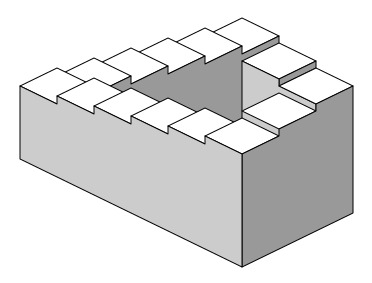
\includegraphics[width=0.5\textwidth]{impossible_staircase.jpg}
    \caption{Penrose steps diagram from Wikipedia - By Sakurambo - Own work, Public Domain, https://commons.wikimedia.org/w/index.php?curid=794844}
    \label{fig:penrose}
\end{figure}
The penrose steps are an architectural paradox that creates the illusion of an infinite staircase.\footnote{Christopher Nolan famously reconstructed this illusion in his film Inception (2010). If you are interested, the scene can be found \href{https://www.youtube.com/watch?v=BjLzIfDpGhs}{here} and behind the scenes \href{https://youtu.be/HzdK_JC2BE4}{here}.} The steps appear to be continuously ascending or descending, but in reality, they form a closed loop. This paradox is achieved through clever use of perspective and geometry, creating an optical illusion that tricks the viewer's perception of space.


\subsection{Mobius Strip}\index{mobius strip}

% could be wrap fig
% https://tex.stackexchange.com/questions/118563/moebius-strip-using-tikz 
\begin{figure}[H]

    \centering
% Source - https://tex.stackexchange.com/a/118573
% Posted by Jake, modified by community. See post 'Timeline' for change history
% Retrieved 2026-03-30, License - CC BY-SA 3.0

        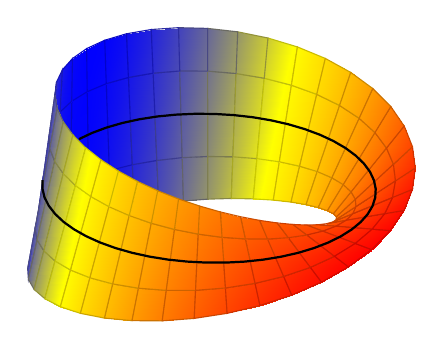
\begin{tikzpicture}
        \begin{axis}[
            hide axis,
            view={40}{40}
        ]
        \addplot3 [
            surf, shader=faceted interp,
            point meta=x,
            colormap/hot,
            samples=40,
            samples y=5,
            z buffer=sort,
            domain=0:360,
            y domain=-0.5:0.5
        ] (
    {1.5*(1+0.5*y*cos(x/2))*cos(x)},
            {(1+0.5*y*cos(x/2)))*sin(x)},
            {0.5*y*sin(x/2)});

        \addplot3 [
            samples=50,
            domain=-145:180, 
            samples y=0,
            thick
        ] (
            {1.5 * cos(x)},
            {sin(x)},
            {0});
        \end{axis}
        \end{tikzpicture}
        \caption{A parametric graph of a mobius strip.}
    \label{fig:mobius}
\end{figure}

The mobius strip is a piece of paper is a \textit{surface} that is said to have one side and one boundary. It is formed most easily (you can do this at home!) by taking a strip of paper, giving it a half twist, and then taping the ends together. The resulting shape is a non-orientable surface, meaning that it has only one side and one edge. If you were to start drawing a line down the middle of the strip, you would find that you return to your starting point after traversing the entire length of the strip, without ever lifting your pen. There is no \textit{inside} or \textit{outside} to the mobius strip. 

If you are curious, the mobius strip is defined by the following parametric equations:
$$\mathbf{r}(u,v) =
\bigl(
(1 + v\cos \tfrac{u}{2})\cos u,\;
(1 + v\cos \tfrac{u}{2})\sin u,\;
v\sin \tfrac{u}{2}
\bigr)$$
where $u$ ranges from $0$ to $2\pi$ and $v$ ranges from $-1$ to $1$.
\subsection{Coastline paradox}
The \newterm{coastline paradox} highlights an issue in measuring irregular geometric objects; their length is changes under changes in measurement scale. Unlike smooth curves in classical Euclidean geometry, natural coastlines exhibit intricate, self-similar structure across many scales. As the measuring unit becomes smaller, more of this fine structure is resolved, and the total measured length increases. This originated in the 1950's when a Lewis Fry Richardson was researching how border lengths could effect the likelihood of war, and there was a discrepancy between the Portuguese measurement of Spain's border compared to the Spanish. Simply, the shorter the unit (or ruler), the longer the measured border; the Spanish and Portuguese geographers were simply using different rulers. However, as the ``ruler length'' approaches zero, the length grows infinity, rather than approaching a finite value!

ADD: Diagram from tikz of coastline

This phenomenon contradicts with calculus and its ideas on the definition of arc length. In calculus, the length of a curve ($y = f(x)$) over an interval is defined as the definite integral $\int f(x)\, dx$ between two points, which often leads to a finite value for smooth or simple functions. The coastline paradox demonstrates that this limiting process fails for highly irregular sets; the coastlines are not ``smooth'' enough. Consequently, arc length integrals cannot be utilized, and alterative methodologies are used to find the length of these areas, termed fractal surface perimeters.

%  \subsection{Ship of Thesus}
% leaving this out for now but could add in future - Arjan, April 2026
 
